\subsection{Ablation study for GCF}
\textcolor{red}{For GCF we have used the wrong adjacency matrix, that do not contain self connections. We are unsure what the difference will be in the result, but the results might change.}
Meng Liu et. al does not present an ablation study for BiTGCF and GCF, which LightGCN showed is important with their regards to NGCF \cite{lightgcn,BiTGCF}.
In this section we conduct an ablation study on GCF to get an understanding on the effect of the different parts of the embedding propagation and layer combination.
\autoref{fig:GCF-NDCG-ablation-study} and \autoref{fig:GCF-recall-ablation-study} contains the GCF ablation study, where all GCF modifications still have the inner product between users and items, except for LightGCN.
The methods are as described here:\\
\textcolor{red}{(We might also be required to test this with dropout to prevent overfitting on the methods that utilizes concatenation as layer combination, and see what effect this has on the results.)}
\begin{itemize}
    \item \textbf{GCF}: The original GCF method as described in \autoref{subsubsec:GCF-embed-propagation}.
    \item \textbf{GCF-sum}: GCF where the layer combination has been changed to weighted summation instead of concatenation.
    \item \textbf{GCF-only-IP}:  GCF where $e_i^{(k)}$ has been removed in \autoref{eq:GCF-embedding}, so that GCF's graph convolutions only considers the inner product of users and items.
    \item \textbf{GCF-sum-only-IP}: Implemented as GCF-only-IP except that the layer combination method used is weighted summation.
    \item \textbf{GCF-minus-IP}: GCF where inner product has been removed. \textcolor{red}{results missing}
    \item \textbf{LightGCN}: Original LightGCN as described in \autoref{subsubsec:LightGCN-embed-propagation}.
    \item \textbf{LightGCN-concat}: LightGCN with concatenation as layer combination. \textcolor{red}{results missing}
\end{itemize}

\begin{figure}[h!]
    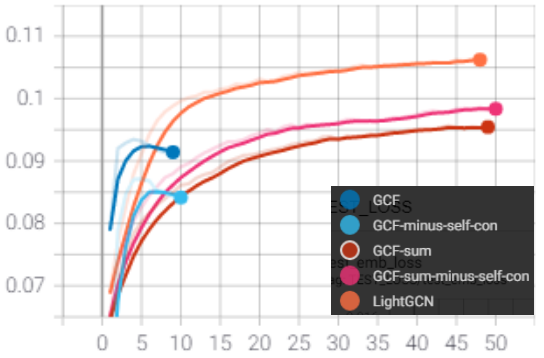
\includegraphics[width=\linewidth]{figures/GCF-NDCG-Yelp-ablation.png}
    \caption{NDCG@50 for the Yelp2020 dataset.}
    \label{fig:GCF-NDCG-ablation-study}
\end{figure}

\begin{figure}[h!]
    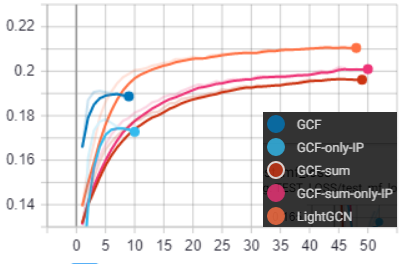
\includegraphics[width=\linewidth]{figures/GCF-recall-Yelp-ablation.png}
    \caption{Recall@50 on the Yelp2020 dataset.}
    \label{fig:GCF-recall-ablation-study}
\end{figure}
From \autoref{fig:GCF-NDCG-ablation-study} and \autoref{fig:GCF-recall-ablation-study} it can be seen that the methods that do utilize concatenation as layer combination performs worse than the methods that utilize summation.
For these experiments the dropout ratio is 0, so it could be because the concatenation methods hits overfitting.
Additionally we can see that convolutions of items and user are beneficial, when using concatenation as layer combination, but decreases performance when using weighted summation as layer combination, while combining it with inner product.
This is likely because weighted summation is more sensitive to changes in the embedding, and using both neighboring convolutions and inner product can create contradictions.
